\documentclass[12pt,fleqn]{article}\usepackage{../../common}
\begin{document}
Eğrilik (Curvature)

Bir eğrimiz var, bu eğriye herhangi bir noktada ona en iyi uyan, onun eğimini en
iyi gösteren bir çemberi nasıl buluruz? Alttaki gibi bir uyumdan bahsediyoruz,

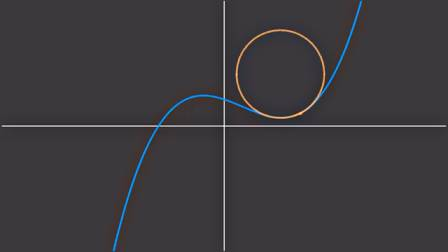
\includegraphics[width=15em]{calc_multi_60_01.jpg}

Bu yazıda bu ideal çemberin yarıçapını bulmayı göreceğiz, elde edilecek
formül eğrinin o noktadaki türevleri üzerinden yapılacak.

Çemberin bir $x_0,y_0$ merkezli olduğunu düşünelim, ve yarıçapı $r$ olsun. Bu
çemberin formülü şekildeki gibi olur,

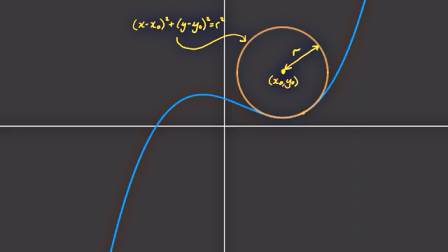
\includegraphics[width=15em]{calc_multi_60_02.jpg}

Şimdi cebirsel numaralara gelelim. Çember 

$$
(x-x_0)^2 + (y-y_0)^2 = r^2
$$

formülünün $x$'e göre türevini alalım. Karedeki 2 aşağı iner, ve parantez içinin
türevi alınır,

$$
2 (x-x_0) [1] + 2(y-y_0) \frac{\ud y}{\ud x} = 0
$$

$$
(x-x_0) + (y-y_0) \frac{\ud y}{\ud x} = 0
$$

Şimdi üstteki formülün bir kez daha türevini alalım,

$$
1 + (y-y_0) \frac{\ud^2y}{\ud x^2} +
\left(  \frac{\ud y}{\ud x}  \right) \frac{\ud y}{\ud x}  = 0
$$

$$
1 + (y-y_0) \frac{\ud^2y}{\ud x^2} +
\left(  \frac{\ud y}{\ud x}  \right)^2 = 0
$$

Böylece çember formülünden başlayarak üç tane formül elde etmiş olduk.

$$
(x-x_0)^2 + (y-y_0)^2 = r^2
\mlabel{1}
$$

$$
(x-x_0) + (y-y_0) \frac{\ud y}{\ud x} = 0
\mlabel{2}
$$

$$
1 + (y-y_0) \frac{\ud^2y}{\ud x^2} +
\left(  \frac{\ud y}{\ud x}  \right)^2 = 0
\mlabel{3}
$$

[devam edecek]

Kaynaklar

[1] Radius of Curvature Proof - approximating a curve with a circle!,
    \url{https://www.youtube.com/watch?v=ZCJfq77sFE8}

\end{document}
